% Compile: pdfLaTeX (or LuaLaTeX). Overleaf-friendly.
% Investigation: AMD ROCm product page vs our CUDA-to-HIP porting work.
\documentclass[aspectratio=169,11pt]{beamer}

\usetheme{Madrid}
\usecolortheme{whale}
\setbeamertemplate{navigation symbols}{}
\setbeamertemplate{footline}[frame number]
\setbeamerfont{title}{size=\Large\bfseries}
\setbeamerfont{frametitle}{size=\large\bfseries}

\usepackage{booktabs}
\usepackage{tikz}
\usetikzlibrary{arrows.meta,positioning}

\title{ROCm vs Our CUDA$\rightarrow$HIP Work}
\subtitle{Is AMD's ROCm offering competition --- or the platform we stand on?}
\author{Konstantin Kolchin}
\date{28 July 2026}

\begin{document}

%----- title -----
\begin{frame}
  \titlepage
  \vspace{0.4em}
  \begin{center}
    \small
    Sources: \url{amd.com/en/products/software/rocm},\\
    \url{rocm.docs.amd.com}, ROCm-DS / hipVS docs (2026).
  \end{center}
\end{frame}

%----- verdict -----
\begin{frame}{Verdict (one slide)}
  \begin{block}{Not competition --- \textbf{substrate}}
    ROCm is AMD's open GPU software stack (runtime, compilers, math/AI libs,
    HIP/HIPIFY). Our CUDA$\rightarrow$HIP projects \textbf{consume} that stack
    and deliver \textbf{product-path} ports (Milvus / Knowhere / hipVS on
    RDNA3) that ROCm alone does not ship.
  \end{block}

  \vspace{0.5em}
  \begin{columns}[T]
    \begin{column}{0.48\textwidth}
      \begin{block}{Where ROCm competes}
        \footnotesize
        Against \textbf{NVIDIA CUDA} as a
        customer platform choice
        (PyTorch, vLLM, Instinct).
      \end{block}
    \end{column}
    \begin{column}{0.48\textwidth}
      \begin{block}{Where we compete}
        \footnotesize
        Against ``stay on CUDA'' /
        ``wait for upstream'' ---
        we close \textbf{integration +
        gfx1100 + measurement} gaps.
      \end{block}
    \end{column}
  \end{columns}
\end{frame}

%----- what ROCm is -----
\begin{frame}{What AMD sells as ``ROCm''}
  \footnotesize
  From AMD / ROCm docs (Core SDK framing):

  \begin{itemize}
    \item \textbf{Platform:} HIP runtime + compilers (\texttt{amdclang++} / \texttt{hipcc})
    \item \textbf{Porting aids:} HIPIFY (\texttt{hipify-clang}, \texttt{hipify-perl})
    \item \textbf{Libraries:} hipBLAS / rocBLAS, MIOpen, RCCL, hipCUB, \ldots
    \item \textbf{AI / DS:} framework wheels (PyTorch,\ldots);
          ROCm-DS (\textbf{hipRAFT}, \textbf{hipVS}, hipDF,\ldots)
    \item \textbf{Tools:} rocprofiler, ROCgdb, AMD SMI
  \end{itemize}

  \vspace{0.4em}
  \begin{block}{Marketing intent}
    \footnotesize
    Make AMD GPUs a credible alternative to CUDA for HPC and AI ---
    \textbf{not} a turnkey ``port Milvus for you'' service.
  \end{block}
\end{frame}

%----- stack diagram -----
\begin{frame}{Where our work sits}
  \centering
  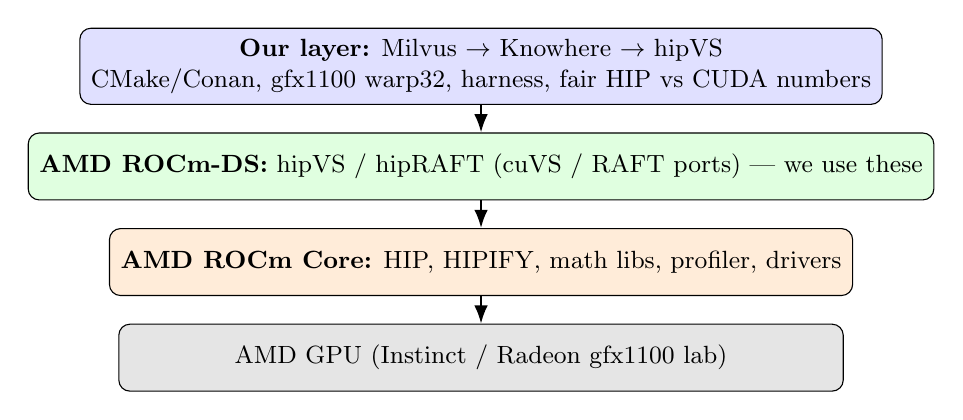
\begin{tikzpicture}[
    box/.style={draw,rounded corners,align=center,font=\small,
                 minimum width=9.2cm,minimum height=0.85cm,inner sep=4pt},
    font=\small,
  ]
    \node[box,fill=blue!12] (prod)
      {\textbf{Our layer:} Milvus $\rightarrow$ Knowhere $\rightarrow$ hipVS\\
       CMake/Conan, gfx1100 warp32, harness, fair HIP vs CUDA numbers};
    \node[box,fill=green!12,below=0.35cm of prod] (ds)
      {\textbf{AMD ROCm-DS:} hipVS / hipRAFT (cuVS / RAFT ports) --- we use these};
    \node[box,fill=orange!15,below=0.35cm of ds] (core)
      {\textbf{AMD ROCm Core:} HIP, HIPIFY, math libs, profiler, drivers};
    \node[box,fill=gray!20,below=0.35cm of core] (hw)
      {AMD GPU (Instinct / Radeon gfx1100 lab)};
    \draw[-Latex,thick] (prod) -- (ds);
    \draw[-Latex,thick] (ds) -- (core);
    \draw[-Latex,thick] (core) -- (hw);
  \end{tikzpicture}

  \vspace{0.35em}
  {\footnotesize Overlap with ROCm is \textbf{intentional dependency}, not rivalry.}
\end{frame}

%----- overlap table -----
\begin{frame}{Overlap map}
  \footnotesize
  \begin{center}
  \begin{tabular}{@{}p{3.2cm}p{4.0cm}p{4.0cm}@{}}
    \toprule
    \textbf{Capability} & \textbf{ROCm / AMD ships} & \textbf{Our projects add} \\
    \midrule
    CUDA$\rightarrow$HIP syntax & HIPIFY + HIP API & Apply + debug in large trees \\
    Vector search lib & hipVS (cuVS port) & Wire into Knowhere/Milvus \\
    Math / DL kernels & hipBLAS, MIOpen,\ldots & Use as deps; rare patches \\
    RDNA3 / warp32 & Partial / experimental & Make FLAT/PQ product path work \\
    Product (Milvus) & Not a ROCm deliverable & Standalone HIP build + seal \\
    Fair peer numbers & Not their job & Layer-4 / lib / GIST recipes \\
    \bottomrule
  \end{tabular}
  \end{center}
\end{frame}

%----- hipVS -----
\begin{frame}{hipVS is AMD's --- we harden the product path}
  \begin{itemize}
    \item hipVS = official ROCm-DS port of RAPIDS \textbf{cuVS}
          (API-aligned; C++/Python/\ldots).
    \item That \textbf{reduces} library-port work vs writing ANN from scratch.
    \item It does \textbf{not} replace:
          \begin{itemize}
            \item Knowhere CMake / Conan / logger / OpenMP glue
            \item Milvus Standalone HIP bring-up
            \item gfx1100 \texttt{USE\_WARPSIZE\_32} + IVF correctness
            \item Catch2 gaps (e.g.\ CAGRA) and peer-GPU measurement
          \end{itemize}
  \end{itemize}

  \vspace{0.4em}
  \begin{block}{Implication}
    \footnotesize
    Upstream ROCm-DS success \textbf{helps} us (better library).
    It does not obsolete the integration / RDNA3 / benchmark layers.
  \end{block}
\end{frame}

%----- real competitors -----
\begin{frame}{Who actually competes with our porting work?}
  \begin{enumerate}
    \item \textbf{Stay on NVIDIA} --- CUDA Milvus / cuVS ``just works'';
          no port cost.
    \item \textbf{Wait for AMD upstream} --- hope hipVS + future Milvus AMD
          images cover the product (Instinct-first; RDNA3 last).
    \item \textbf{Drop-in translators} (e.g.\ ZLUDA-class) --- claim run CUDA
          binaries on AMD \textbf{without} a real HIP port
          (fragile; not our strategy).
    \item \textbf{Rewrite / CPU-only} --- skip GPU ANN on AMD.
  \end{enumerate}

  \vspace{0.45em}
  {\footnotesize ROCm is the shared toolkit for options 2--3 and for us ---
   not a rival project in the same delivery lane.}
\end{frame}

%----- HIPIFY limits -----
\begin{frame}{HIPIFY is necessary, not sufficient}
  \footnotesize
  AMD messaging: HIP mirrors CUDA; HIPIFY automates many API renames.

  \vspace{0.35em}
  \textbf{Still manual / project-specific (our experience):}
  \begin{itemize}
    \item Build systems (CMake, Conan, dual CUDA/HIP flags)
    \item Libraries without 1:1 maps (or ``hip'' vs ``roc'' choices)
    \item Inline PTX / arch assumptions / warp size
    \item Product semantics (sealed indexes, QueryNode path)
    \item Performance parity measurement on peer GPUs
  \end{itemize}

  \vspace{0.35em}
  \begin{block}{One line}
    HIPIFY gets you \emph{compiling candidates}.\\
    Our layers get you a \emph{shippable Milvus GPU path on gfx1100}.
  \end{block}
\end{frame}

%----- strategic -----
\begin{frame}{Strategic read for management}
  \begin{itemize}
    \item \textbf{Invest in ROCm fluency} --- it is the only official AMD path;
          ignore it and the port dies.
    \item \textbf{Do not position our work as ``alternative to ROCm''} ---
          position as \textbf{product enablement on ROCm}.
    \item \textbf{Differentiation:} RDNA3 lab reality, Milvus/Knowhere depth,
          fair HIP vs CUDA science (SIFT / GIST / lib benches).
    \item \textbf{Watch upstream:} ROCm-DS hipVS GA reduces library risk;
          CAGRA / Instinct-first still leave consumer-GPU product work.
  \end{itemize}
\end{frame}

%----- takeaway -----
\begin{frame}{Takeaway}
  \begin{center}
    \Large
    ROCm competes with \textbf{CUDA}.\\[0.35em]
    {\normalsize Our CUDA$\rightarrow$HIP projects compete with
     \textbf{not porting} (or waiting).}\\[0.6em]
  \end{center}

  \begin{block}{Bottom line}
    Extent of competition with our work: \textbf{low / complementary}.\\
    Extent of dependence: \textbf{high} --- ROCm + hipVS are prerequisites.\\
    Value we add: product integration, RDNA3 hardening, measurement.
  \end{block}

  \vspace{0.4em}
  {\footnotesize
  Refs: AMD ROCm product page; \texttt{rocm.docs.amd.com} (What is ROCm?, HIP porting);
  \texttt{ROCm-DS/hipVS}. Lab context: Milvus GPU$\rightarrow$AMD Layers 0--4.}
\end{frame}

\end{document}
